\documentclass[a4paper,11pt]{article}
\usepackage[T1]{fontenc}
\usepackage[utf8]{inputenc}
\usepackage{amsmath}
\usepackage{amsfonts}

\usepackage{lmodern}
\usepackage{footnote}
\usepackage{graphicx}
\usepackage{subfig}
\usepackage[italian]{babel}
\usepackage[hidelinks]{hyperref}
\usepackage{subfig}
\usepackage{listings} % formattazione codice
\usepackage{verbatim}

\usepackage{parskip}

\usepackage{tikz}

\title{Confronto Funzioni Hash}
\author{Niccolò Boanini}
\date{}

\begin{document}

\maketitle
\tableofcontents

\begin{abstract}
Questo esercizio di Laboratorio ha come obiettivo quello di porre a confronto il metodo della divisione con il metodo della moltiplicazione per calcolare la funzione hash $h(k)$, utilizzando il concatenamento come regola per gestire le eventuali collisioni.
\end{abstract}

\section{Metodi utilizzati per il calcolo di \boldmath\texorpdfstring{$h(k)$}{h(k)}} \label{metodi}

% % % % % % % % % % % % % % % % % % M. DIVISIONE
\subsection{Metodo della divisione} \label{metodo_div}
Il metodo della divisione permette di calcolare l'hash come il resto della divisione tra una chiave $k$ e un determinato $m$ che rappresenta la dimensione della tabella.

La funzione hash utilizzata è la seguente: 
\begin{equation}
    \label{eq:metodo_div}
    \boxed{h(k)= k \text{ mod }  m}
\end{equation}

$Nota$: Risulta influente al fine di limitare le collisioni scegliere come $m$ un numero primo non vicino a una potenza di $2$.

% % % % % % % % % % % % % % % % % % M. MOLTIPLICAZIONE
\subsection{Metodo della moltiplicazione}
\label{metodo_mol}
Il metodo della moltiplicazione calcola l'hash utilizzando la funzione qui di seguito:
\begin{equation}
    \label{eq:metodo_mol}
    \boxed{h(k)= \lfloor m \ (kA \text{ mod } 1) \rfloor}
\end{equation}
In pratica viene estratta la parte frazionaria di $kA$ (con $A \in (0;1)$ una costante da scegliere\footnote{L'informatico statunitense Knuth raccomanda $A \approx \varphi^{-1} = (\sqrt{5}-1)/2 = 0,618033...$ , ovvero l'inverso della $sezione \ aurea$ \cite{fibo_hash} \label{knuth_value} }), quindi viene moltiplicata per $m$ e infine prelevata la parte intera inferiore.

$Nota$: a differenza di \eqref{eq:metodo_div} in questo caso il valore di $m$ non è critico. Ciò detto, tipicamente si pone $m=2^{p} \ , \ p \in \mathbb{N}$  (ossia come potenza intera di $2$).
\section{Descrizione del lavoro svolto} \label{descr_lavoro}

Per completare l'esercizio sono stati effettuati diversi test volti a evidenziare il comportamento delle tabelle a seconda di specifici dati in ingresso.

L'approccio seguito in primo luogo è stato quello del \textit{worst case analysis}, volto a studiare cioè l'evoluzione delle tabelle hash quando in ingresso vengono inseriti i dati considerati appunto \textit{peggiori} per i relativi metodi.
\\ Successivamente lo studio si è concentrato su una analisi più generale e casuale, con l'obiettivo di riassumere al meglio i vantaggi e gli svantaggi di ogni metodo quando in input si hanno dati non predicibili.
\\Osserveremo allo stesso tempo il progressivo riempimento della tabella man mano che cresce il \textit{load factor} $\alpha$.

\subsection{Sviluppo e implementazione dei metodi}
I test sono stati effettuati in \verb|Python v3.10| utilizzando \verb|Matplotlib| come libreria per la creazione dei grafici.
\\Al fine di confrontare al meglio i due metodi è stata creata una tabella apposita per ognuno: \verb|T1| è riempita da oggetti della classe \verb|User| attraverso il metodo della divisione; \verb|T2| ospita i medesimi oggetti della classe \verb|User| ma questi sono inseriti sfruttando il metodo della moltiplicazione\footnote{In alcuni esempi (come il \ref{worst_case_mol}), sono state utilizzate più di due tabelle per completare il confronto}.
\\ Ogni oggetto è composto dall'abbinamento degli attributi \verb|key| e \verb|value|, dove quest'ultimo è un identificatore \textit{human-readable}, cioè una stringa caratteristica dell'oggetto stesso (facoltativo ai fini degli esperimenti ma utile per la comprensione e per possibili implementazioni più complesse).
\\ Le principali funzioni del programma sono:
\begin{itemize}
    \item \verb|func_div(key)| e \verb|func_mul(key)|: Funzioni hash
    \item \verb|insert(User)|: Inserimento simultaneo di un utente in \verb|T1| e \verb|T2|
    \item \verb|delete(User)|: Rimozione di un utente da \verb|T1| e \verb|T2|
    \item \verb|searchT1(key)|: Ricerca chiave in \verb|T1| (analoga per \verb|T2|)
    \item \verb|print_all()|: Visualizzazione su console delle tabelle, del \textit{load factor} e del numero di collisioni rilevate su ciascuna tabella
    \item \verb|plt.show()|: Visualizzazione dei grafici sulla GUI di \verb|Matplotlib|
\end{itemize}


\subsection{Ipotesi}
Le ipotesi che assumeremo vere sono le seguenti:
\begin{enumerate}
    \item[i.] Non possono esserci due \verb|User| con la stessa chiave;
    \item[ii.] Le collisioni sono gestite con il \textit{concatenamento};
    \item[iii.] Le tabelle hanno tutte la stessa dimensione $m$.
\end{enumerate}



\begin{comment}
    \lstset{
      basicstyle=\footnotesize,
      xleftmargin=.3\textwidth, xrightmargin=.2\textwidth
    }
    \begin{lstlisting}
        insert(T,100,"Greco")
    \end{lstlisting}
    
    Abbiamo poi ottenuto il seguente grafico che mostra...
    
    \begin{figure}[htb]
    \begin{center}
    \includegraphics[scale=0.5]{src/img/graph1.pdf}
    \caption{This is a figure.}
    \end{center}
    \end{figure}
\end{comment}
\section{Risultati attesi} \label{ris_attesi}
Dalle implicazioni teoriche che abbiamo esposto in particolare nella sezione \ref{metodo_div} ci aspettiamo che il metodo della divisione produca dei risultati negativi (ovvero numerose collisioni) quando $m$ è una potenza intera di due oppure per come è definita $h(k)$ quando abbiamo tanti valori delle chiavi $k$ che sono multipli di $m$.
\\Risulta invece difficile prevedere a priori l'esatta evoluzione della tabella quando si utilizza il metodo della moltiplicazione. Sappiamo però che qualsiasi valore di $A \in (0;1)$ è sufficiente buono, anche se quello di Knuth sembra il più appropriato \cite{textbook}\cite{fibo_hash}.

Per quanto riguarda in generale il \textit{load factor}, ci aspettiamo che esso influisca sulle prestazioni quando diventa un valore superiore al $75 \%$ \cite{wikipedia}.
\section{Risultati ottenuti} \label{ris_ottenuti}
Di seguito vengono presentati e analizzati i test eseguiti, uno per volta.

% 1
\subsection{Caso peggiore metodo divisione} \label{caso_peggiore_div}
Seguendo la filosofia \textit{worst case analysis}, osserviamo il comportamento della tabella quando sono assegnati i valori critici per il metodo della divisione. \\
Impostiamo quindi: $m = 2^{p}$ (in questo caso $m = 16$) e tutte le chiavi $k$ degli utenti \verb|User| tra loro multiple di $m$, ovvero ad esempio $16,32,48,64$ etc.
Inseriamo in tutto $11$ oggetti in tabella così da avere alla fine come \textit{load factor} $\alpha = n/m \approx 70\%$.

Possiamo eseguire il tutto con il seguente \textit{snippet} di codice che invocherà i metodi implementati:

% multiline code snippet
\lstset{
      basicstyle=\small,
      xleftmargin=.1\textwidth,
}
\begin{lstlisting}
key = m
for i in range(11):
    Hash.insert(User(key, string.ascii_uppercase[i]))
    key + = m
\end{lstlisting}


In questo modo tutti gli oggetti hanno come chiave \verb|key| un multiplo di $m$ e come attributo \verb|value| una lettera dell'alfabeto (da \verb|"a"| fino a \verb|"k"| essendoci in tutto $11$ elementi).

\begin{figure}[htb]
    \begin{center}
    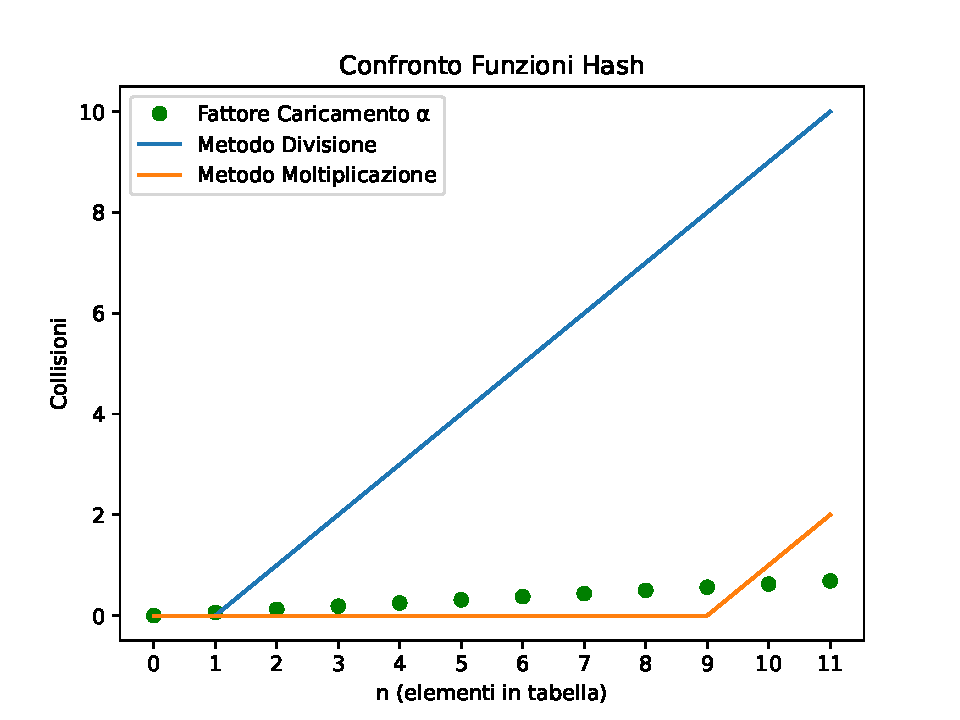
\includegraphics[scale=0.65]{src/img/worstcase.pdf}
    \caption{Caso peggiore metodo della divisione}
     \label{fig:met_div}
    \end{center}
\end{figure}

Come si nota in Figura \ref{fig:met_div}, il metodo della divisione risulta pessimo: dopo il primo elemento inserito, abbiamo tutte e sole collisioni.
\\ Viceversa il metodo della moltiplicazione grazie alla sua funzione di hash apparentemente casuale riesce a gestire assai meglio la situazione, e si rilevano due sole collisioni rispettivamente quando si inserisce il decimo e l'undicesimo elemento. In Figura \ref{fig:tikz:worstcase} è riportata la struttura grafica della tabella.

\begin{figure}[htp]
  Tabella T1 (metodo divisione):

\begin{tikzpicture}
\coordinate (0);
\foreach \t/\n[count=\i from 0,evaluate=\i as\j using int(\i+1)] in {
 K $\rightarrow$ J $\rightarrow$ I $\rightarrow$ H $\rightarrow$ G $\rightarrow$ F $\rightarrow$ E $\rightarrow$ D $\rightarrow$ C $\rightarrow$ B $\rightarrow$ A/ ,
 ,
 ,
 ,
 ,
 ,
 ,
 ,
 ,
 ,
 ,
 ,
 ,
 ,
 ,
}
\node at(\i.south)[anchor=north,draw,minimum height=1.4em,minimum width=2.5em,outer sep=0pt](\j){\n}
    node at(\j.west)[align=right,left]{\i} 
    node at(\j.east)[align=left,right,xshift=-.7em]{$\rightarrow$ \t};
\end{tikzpicture}

\vspace{20pt}
Tabella T2 (metodo moltiplicazione):

\begin{tikzpicture}
\coordinate (0);
\foreach \t/\n[count=\i from 0,evaluate=\i as\j using int(\i+1)] in {
 ,
 H/,
 ,
 G/,
 ,
 F/,
 ,
 E/,
 D/,
 ,
 C/,
 ,
 K $\rightarrow$ B/,
 ,
 J $\rightarrow$ A/,
 I/
}
\node at(\i.south)[anchor=north,draw,minimum height=1.4em,minimum width=2.5em,outer sep=0pt](\j){\n}
    node at(\j.west)[align=right,left]{\i} 
    node at(\j.east)[align=left,right,xshift=-.7em]{$\rightarrow$ \t};
\end{tikzpicture}

\newpage
  \caption{Le due tabelle del caso \ref{caso_peggiore_div} a confronto.}
  \label{fig:tikz:worstcase}
\end{figure}

\textit{Nota}: l'andamento delle collisioni con il metodo della moltiplicazione cresce in modo lineare (quindi critico) dopo che il \textit{load factor} supera i valori massimi di riferimento. Motivo per il quale in questi casi è consigliato ridimensionare la tabella, ad esempio raddoppiando il valore di \textit{m}.

%2
\subsection{Caso peggiore metodo moltiplicazione (?)} \label{worst_case_mol}
Come già descritto nella sezione \ref{metodo_mol}, il metodo della moltiplicazione soffre apparentemente di meno criticità. L'unico parametro che possiamo variare per capire se influisce o meno sulle prestazioni è $A$. Come si dimostra negli esempi successivi tuttavia, qualsiasi valore compreso tra $0$ e $1$ è sufficientemente buono, anche se basta distaccarsi di poco dal valore di Knuth\footref{knuth_value} per ottenere risultati sensibilmente differenti.


Utilizzando gli stessi dati di \ref{caso_peggiore_div}, analizziamo le varie evoluzioni della tabella al variare di $A$. In particolare si pone:
\[
\overbrace{A=(\sqrt{5}-1)/2 = 0,618033...}^{\text{Knuth}} \quad , \quad \overbrace{A=0,848, \quad , \quad A=0,126}^{\text{valori casuali } \in (0;1)}
\]

\begin{figure}[h]
    \begin{center}
    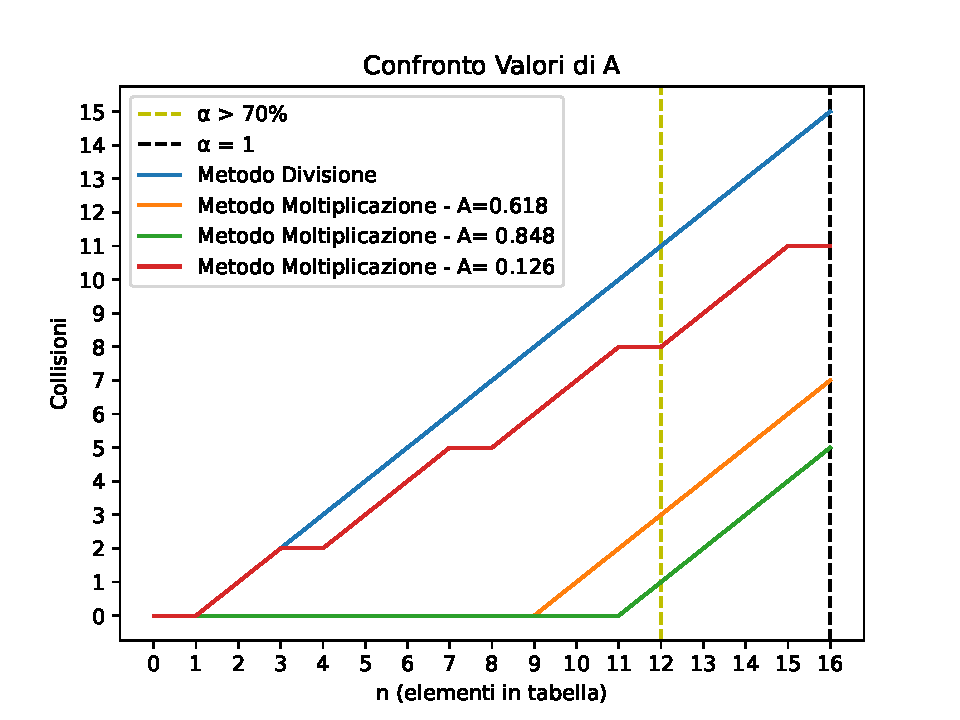
\includegraphics[scale=0.65]{src/img/worstcase_mul.pdf}
    \caption{Evoluzione tabella al variare di $A$}
     \label{fig:worstcase_mul}
    \end{center}
\end{figure}
Il risultato è riportato in Figura \ref{fig:worstcase_mul}. \\ 
Innanzitutto come si nota, tutti e tre i valori utilizzati portano a un risultato migliore rispetto al metodo della divisione in termini di collisioni. \\ 
\'E poi interessante scoprire che ponendo $A = 0.126$ si hanno meno collisioni rispetto al caso $A=(\sqrt{5}-1)/2$. Questo perché il valore di Knuth è \emph{probabilisticamente} migliore, cioè si comporta in generale sempre sufficientemente bene ma in casi specifici ci possono essere alternative migliori. \\
Pertanto complessivamente possiamo dire che non esiste un \emph{caso peggiore} utilizzando il metodo della moltiplicazione, anche se certi valori di $A$ risultano più o meno adatti a seconda dello scenario.
%3
\subsection{Caso randomico}

Confrontiamo adesso i due metodi ponendo in ingresso numerosi valori pseudo-casuali e osserviamo come si comportano le tabelle di conseguenza.

\begin{figure}[p]
\centering
\subfloat{%
  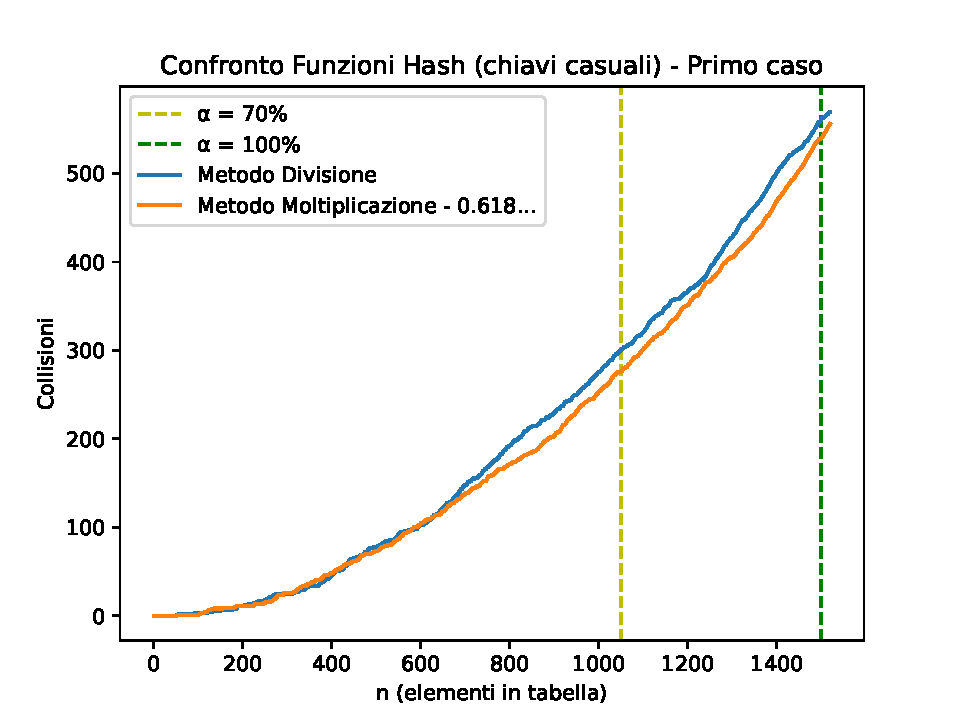
\includegraphics[width=0.67\textwidth]{src/img/CASO1.pdf}%
  } \\
\subfloat{%
  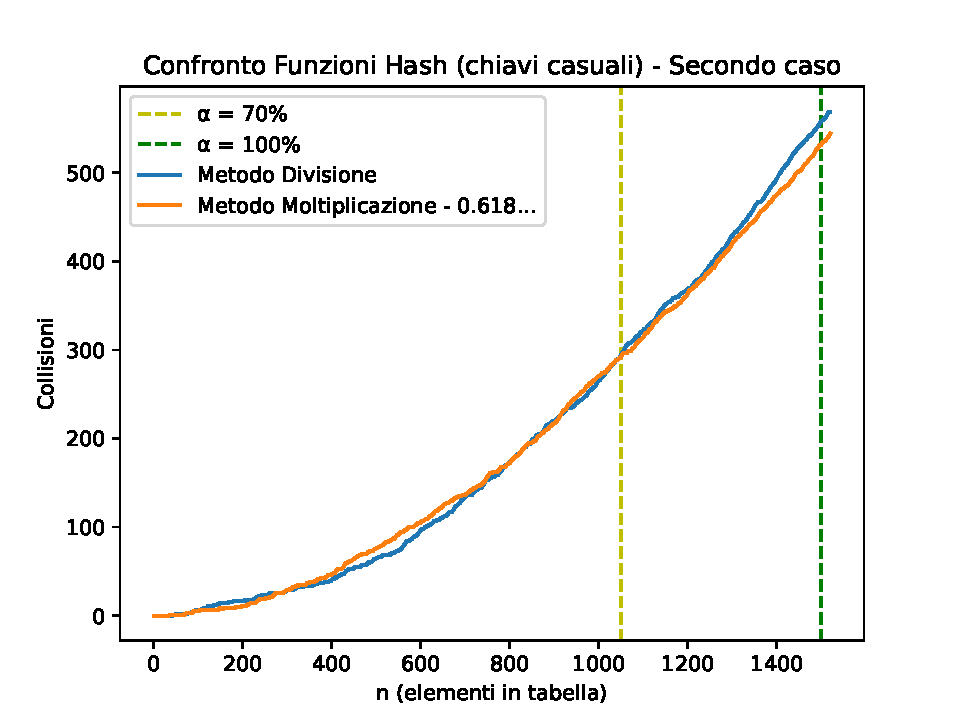
\includegraphics[width=0.68\textwidth]{src/img/CASO2.pdf}%
  }   \\     
\subfloat{%
  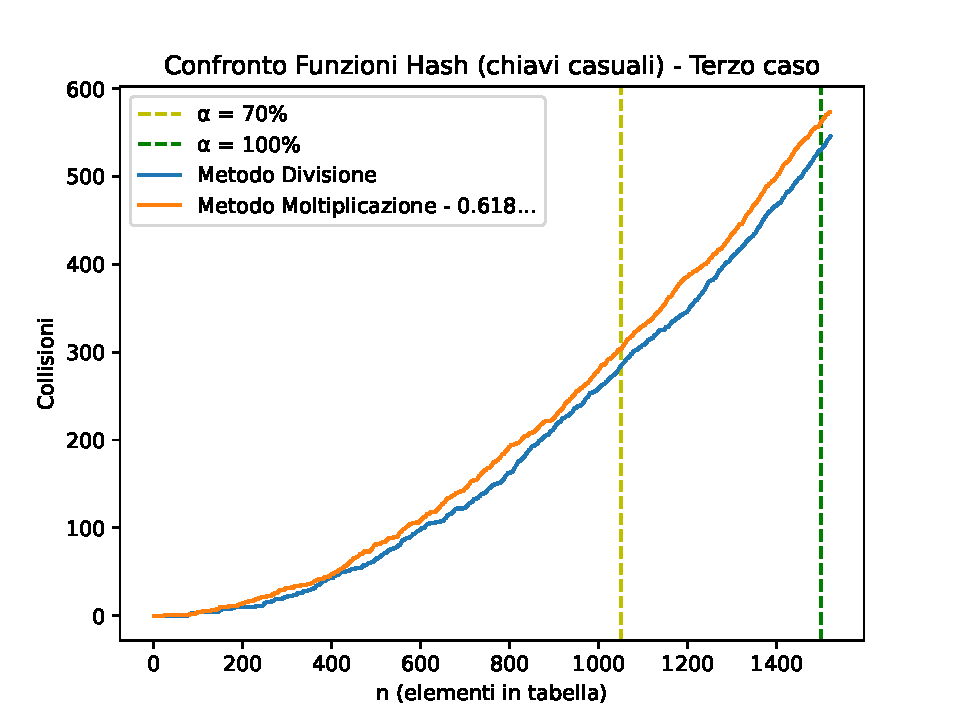
\includegraphics[width=0.68\textwidth]{src/img/CASO3.pdf}%
  } 
\caption{I tre casi a confronto}
\label{fig:random_casi}
\end{figure}

In tutti e tre gli scenari, abbiamo $m = 1500$ e un universo delle chiavi pari a $m \cdot 20=30000$, quindi molto ampio.
Per generare i numeri casuali, sono stati inseriti tutti i numeri da $1$ fino a $m\cdot20$ in una lista sfruttando la funzione \verb|list(range(1,m*20))|, che è stata poi mescolata con la funzione \verb|shuffle| della libreria \verb|random|.
Infine sono stati effettivamente inseriti in tabella i primi $m+20$ elementi\footnote{Un valore a piacimento di poco superiore a $m$ per vedere l'evoluzione della tabella fino (e oltre) $\alpha=100\%$}.
Lo snippet di riferimento è il seguente:
% multiline code snippet
\lstset{
      basicstyle=\small,
      xleftmargin=.1\textwidth,
}
\begin{lstlisting}
tot_ele = m+20
key_universe = list(range(1,m*20))
random.shuffle(key_universe)

for i in range(tot_ele):
	Hash.insert(User(key_universe[i]-1, "i"))
\end{lstlisting}

\textit{Nota}: l'attributo \verb|value| è semplicemente l'indice dell'elemento all'interno della lista (non ha molta importanza).

Passiamo dunque a commentare quanto ottenuto, che è riportato graficamente in Figura \ref{fig:random_casi}.
Notiamo subito la cosa più importante: l'andamento in tutti e tre i (sotto)casi è \textit{simile}: dei due metodi non ce n'è uno predominante. Entrambi causano all'incirca lo stesso numero di collisioni.
\\In dettaglio nel \textit{Primo caso} il metodo della divisione appare leggermente svantaggiante, soprattutto dopo un certo elemento di valori inseriti.
\\ Situazione sostanzialmente di "pareggio" invece nel \textit{Secondo caso}, con i due metodi che in termini di collisioni praticamente si equivalgono.
\\ Infine nel \textit{Terzo caso} risulta lievemente meno performante il metodo della moltiplicazione, nonostante sia stato impostato ad $A$ il valore di Knuth.

Importante sottolineare che se eseguiamo più e più volte il programma, ci ritroviamo sempre in uno dei tre contesti appena esposti, il che ci fa riflettere ancora una volta sull'efficacia e sulle differenze dei metodi. Il tutto sarà descritto completamente nella sezione successiva delle Conclusioni.
\newpage
\section{Conclusioni}

Dagli esperimenti condotti abbiamo avuto come già detto la conferma di certe implicazioni teoriche. Se da una parte il metodo della divisione risulta più semplice da implementare, dall'altra appare vulnerabile a certi dati posti in ingresso. Alcuni di questi possono rendere alcune celle della tabella intasate in poco tempo e appesantire drasticamente l'esecuzione, come visto nell'esempio \ref{caso_peggiore_div}. Questo porta a fare riflessioni soprattutto nell'ambito della sicurezza informatica: un eventuale attacco dall'esterno potrebbe "dirottare" le chiavi degli elementi in ingresso verso i valori critici per il caso specifico, causando le spiacevoli conseguenze suddette. 
\\ D'altro canto il metodo della divisione non è critico rispetto al valore della dimensione della tabella, ma richiede tuttavia una scelta appropriata del valore di $A$. Inoltre l'operazione di moltiplicazione risulta più impegnativa per il calcolatore quando la dimensione della tabella non è una potenza di due ed è nettamente più conveniente l'operazione di divisione quando la tabella ha un numero primo come dimensione (viceversa se la dimensione è una potenza di due l'operazione di moltiplicazione equivale a un semplice AND bit a bit, quindi semplice e veloce in tal caso) \cite{Stack}.

Detto ciò, possiamo dire che su larga scala i due metodi si comportano sostanzialmente allo stesso modo, come abbiamo visto nel caso di Figura \ref{fig:random_casi}, pertanto a seconda delle esigenze si può scegliere l'uno o l'altro. Necessario però sottolineare che oggigiorno esistono metodi e funzioni più avanzate per ridurre le collisioni come l'hash perfetto.
\newpage

\begin{thebibliography}{}

\bibitem{textbook}
T. Cormen, C. Leiserson, R. Rivest, C. Stein, (2010): \emph{Introduzione agli algoritmi e strutture dati}

\bibitem{fibo_hash}
B. Preiss (1998): Data Structures and Algorithms with Object-Oriented Design Patterns - \href{www.google.com}{\emph{Fibonacci Hashing}}

\bibitem{wikipedia}
Wikipedia: \emph{Hash Table}

\bibitem{Stack}
Stack Overflow: \emph{What Are The Disadvantages Of Hashing Function Using Multiplication Method}

\begin{comment}
\bibitem{owolab}
O. Owolab (2003): \emph{Empirical studies of some hashing functions}

\bibitem{maurer_lewis}
W. D. Maurer, T. G. Lewis (1975): \emph{Hash Table Methods}
\end{comment}

\end{thebibliography}



\end{document}
